\section{Methods of Testing Hydrogel Efficacy}

The efficacy of a hydrogel depends on several factors. Absorption, or swelling, tests,
approximated by placing the scaffold in a liquid medium and measuring the percentage increase
in weight. This serves as a measure of permeability, simulating the scaffold's ability to allow cells
and nutrients into the healing area. Stress-strain tests are used to approximate mechanical
strength, ensuring that the hydrogel will not collapse or overextend under mechanical stress.
Adhesion is measured via lap shear or peel tests \autocite{RN5}, which provide a numerical
measure for the ability of the hydrogel to resist movement after its placement. Degradation rate
can be measured in a couple ways, by measuring the overall weight of the scaffold at two or more
points in time. Degradation is measured as a percentage loss in mass or as a
percentage change in the diameter of individual fibrils that make up the matrix. These tests are
effective at measuring individual properties of the matrix ex vivo and predicting the success of
the hydrogel before it is used for treatment. However, an overall test can also be conductive
post-treatment, simply by measuring the strength of the tendon or ligament relative to its original
strength.

\subsection{Biocompatibility}

The Janus Tough Adhesive has shown to exhibit high biocompatibility during testing, despite it containing the synthetic polymer polyacrylamide. To evaluate their performance and impact on natural tissues, \citeauthor{freedmanEnhancedTendonHealing2022} (\citeyear{freedmanEnhancedTendonHealing2022}) experimentally tested  injured and healthy rats, and applied the JTA to the patellar tendon.
For three weeks, potential swelling of the tendon and degredation of the gel were assessed by high frequency ultrasound. When a tendon becomes injured, its echogenicity---the amount of sound it reflects---decreases, because its collagen fibres become more disorganised and less densely packed \autocite{hodgsonTendonLigamentImaging2012}.
Researchers also found that injured tendons without application of the JTA had larger cross-section areas, indicating increased swelling as shown in Figure~\ref{fig:JTA_Patellar_cross_section}. A decrease in inflammation in the affected tendon therefore suggests that the JTA was effective and well-tolerated by the body.
\begin{figure*}[ht]
    \centering
    \begin{minipage}[b]{0.45\textwidth}
        \centering
        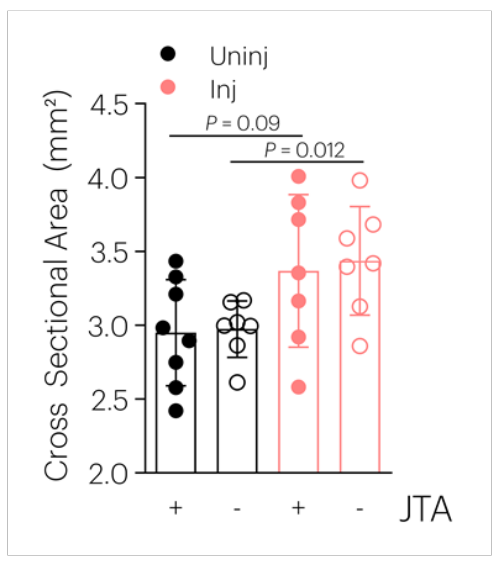
\includegraphics[width=0.6\linewidth]{JTA_cross_section.png}
        \caption{Patellar tendon cross-sectional area (mm\textsuperscript{2}) after 3 weeks of treatment [Adapted from \cite{freedmanEnhancedTendonHealing2022}]}
        \label{fig:JTA_Patellar_cross_section}
    \end{minipage}
    \hfill
    \begin{minipage}[b]{0.45\textwidth}
        \centering
        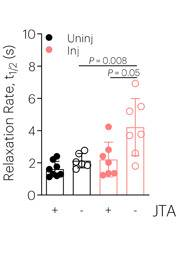
\includegraphics[width=0.6\linewidth]{Figures/JTA_relaxation_patellar.jpeg}
        \caption{Patellar tendon relaxation rate [Adapted from \cite{freedmanEnhancedTendonHealing2022}]}
        \label{fig:JTA_Patellar_relaxation}
    \end{minipage}
\end{figure*}

Furthermore, in the patellar tendon, the JTA was found to have improved tendon relaxation (Figure~\ref{fig:JTA_Patellar_relaxation}), without impacting natural properties such as elastic mechanics, dynamic modulus, or linear modulus.

% Biocompatibility of the JTA was also tested in more complex use cases, such as the rotator cuff and Achilles tendon. 

\subsection{\textit{In vivo} Testing Methods}

Hydrogels can be observed in vivo through various imaging methods including MRI, ultrasound,
and fluorescence. MRIs provide high-resolution contrast that allows researchers to observe
whether the hydrogel remains at the injury site. The swelling of the hydrogel and surrounding
tissues can also be monitored to ensure the hydrogel remains mechanically sound and the
surrounding tissue does not become irritated. Hydrogels are sometimes labeled with contrast
agents like gadolinium to make them more visible. Ultrasound imaging allows for both direct
imaging of the hydrogel and indirect imaging via the effect on adjacent structures. Ultrasound is
particularly beneficial in assessing adherence and in observing the effect of the hydrogel on joint
mobility. In the patellar tendon, the JTA was found to have improved tendon relaxation (Figure~\ref{fig:JTA_Patellar_relaxation}), without impacting natural properties such as elastic mechanics, dynamic modulus, or linear modulus. Fluorescence imaging uses fluorescent tags to track the movement of the hydrogel.
This makes it particularly effective in tracking hydrogel degradation and in visualizing
interactions with adjacent tissues. \citeauthor{freedmanEnhancedTendonHealing2022} showed the effectiveness of imaging
techniques in their rat experiments and also measured the effectiveness of the hydrogel on
recovery. The newly formed rat tendons were removed and tested, showing that the hydrogel
allowed the tendons to recover up to 80\% of their original strength, a marked improvement on
traditional surgical methods.

\subsection{\textit{Ex vivo} Testing Methods}

Ex vivo methods of testing are important to ensure the hydrogel will be effective when it is
placed in the body. Testing should ideally occur under wet conditions to simulate being in an
aqueous body environment. Absorption, or swelling, tests, approximated by placing the network
in a liquid medium and measuring the percentage increase in weight. This serves as a measure
of permeability, simulating the hydrogel's ability to allow cells and nutrients into the healing area.
An ideal hydrogel should fall between 100--500\%, indicating that it can swell enough to allow
cells and nutrients to enter without compromising structural integrity \autocite{zhangProtocolEfficientlyMeasuring2020}. Stress-strain
tests are used to approximate mechanical strength, ensuring that the hydrogel will not collapse
or overextend under mechanical stress. The ultimate tensile strength of the hydrogel should
approximately match the strength of the developing tendon, which falls between the range of
0.5--5 MPa. The Young's modulus of the hydrogel should also fall within a medium range of
about 0.1--10 MPa, ensuring that it remains flexible, while still providing appropriate support of
the tendon \autocite{xiaoMechanicalTestingHydrogels2013}. Adhesion is measured via lap shear or peel tests \autocite{ChenAdvancesApplicationHydrogel}, which
provide a numerical measure for the ability of the hydrogel to resist movement after its
placement. An adhesion strength of anywhere between 5--50 kPa is considered sufficient for
preventing detachment, but not so high to restrict motion or cause trauma. Degradation rate can
be measured in a couple ways, by measuring the overall weight of the scaffold at 2 or more
points in time and representing degradation as a percentage loss in mass or by measuring the
percentage change in the diameter of individual fibrils that make up the matrix. Ideally, the
hydrogel degrades approximately in sync with healing, about 10--30\% within the first month,
before gradually degrading over the next 6--12 months \autocite{zhuTailoringDegradationRates2015}. These tests are effective at
measuring individual properties of the matrix ex vivo and predicting the success of the hydrogel
before it is used for treatment.